
\documentclass[11pt]{article}
\usepackage[margin=0.8in]{geometry}
\usepackage{booktabs}
\usepackage{graphicx}
\usepackage{hyperref}
\usepackage{xcolor}
\usepackage{float}
\hypersetup{colorlinks=true, linkcolor=blue, urlcolor=blue}

\title{TP2-MV-ALiBi Transformer Implementation Report}
\author{SPY American Call TP2 Project}
\date{\today}

\begin{document}
\maketitle

\section{What was implemented}
This stage implements the professor-proposed transformer path on top of the corrected TP2 expiry-label pipeline. The project now has a separate \texttt{TP2MVTransformer/} folder containing: feature-dictionary construction, an MLP ablation, and the first multivariate ALiBi cross-attention transformer.

The transformer does not receive LightGBM predictions, tree leaves, SHAP vectors, or booster scores. Boosting is used only once to identify a stable entry-time feature dictionary \(\mathcal{F}^\star\). The model input is one token per TP2 episode and viable strategy, restricted to \(T1\) and \(K2\). The label is whether the corrected expiry payoff is positive under the \(\$1{,}000\) normalized exposure convention.

\section{Feature dictionary}
The token dataset contains 354,974 strategy tokens from 177,487 unique TP2 episodes. From 149 candidate point-in-time features, the feature discovery stage selected 48 features for \(\mathcal{F}^\star\). The feature blocks are shown in Figure~\ref{fig:blocks}.

\begin{figure}[H]
\centering
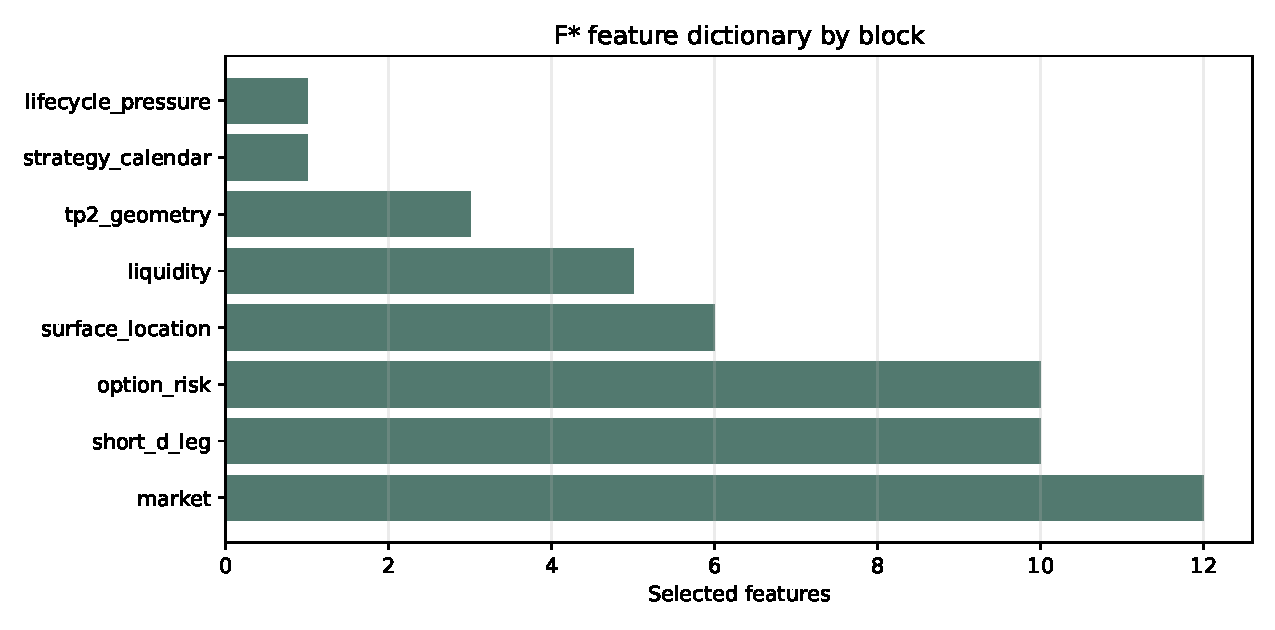
\includegraphics[width=0.86\linewidth]{figures/feature_blocks.pdf}
\caption{Selected transformer feature dictionary by semantic block.}
\label{fig:blocks}
\end{figure}

\section{Rolling evaluation protocol}
All models use the same rolling protocol: train three years, tune threshold on the next validation year, and evaluate once on the next test year. The six test years are 2021--2026. The feature \texttt{signal\_year} is excluded. Future payoff, realized return, holding-period, and label columns are excluded from model inputs.

\section{Model comparison}
\begin{table}[H]
\centering
\small
\begin{tabular}{rrrrrrr}
\toprule
Test year & LightGBM P\&L & LGBM trades & MLP P\&L & MLP trades & MV-ALiBi P\&L & MV trades \\
\midrule
2021 & \$187,760 & 3,019 & \$140,077 & 4,454 & \$2,591,486 & 14,542 \\
2022 & \$39,181 & 499 & \$82,746 & 1,367 & \$-640,596 & 5,023 \\
2023 & \$361,033 & 1,490 & \$683,111 & 1,891 & \$79,309 & 844 \\
2024 & \$171,464 & 5,579 & \$135,139 & 4,908 & \$695,137 & 10,073 \\
2025 & \$688,958 & 5,720 & \$86,127 & 1,947 & \$282,237 & 3,652 \\
2026 & \$224,172 & 672 & \$93,328 & 318 & \$831,608 & 1,220 \\
\bottomrule
\end{tabular}
\caption{Out-of-sample normalized P\&L and selected trades by test year.}
\end{table}

\begin{table}[H]
\centering
\begin{tabular}{lrrr}
\toprule
Model & Total P\&L & Selected trades & Notes \\
\midrule
Corrected LightGBM T1/K2 & \$1,672,567 & 16,979 & current strong tabular benchmark \\
MLP on \(\mathcal{F}^\star\) & \$1,220,529 & 14,885 & no attention context \\
TP2-MV-ALiBi & \$3,839,180 & 35,354 & historical cross-attention \\
\bottomrule
\end{tabular}
\caption{Aggregate normalized P\&L from the saved result tables.}
\end{table}

\begin{figure}[H]
\centering
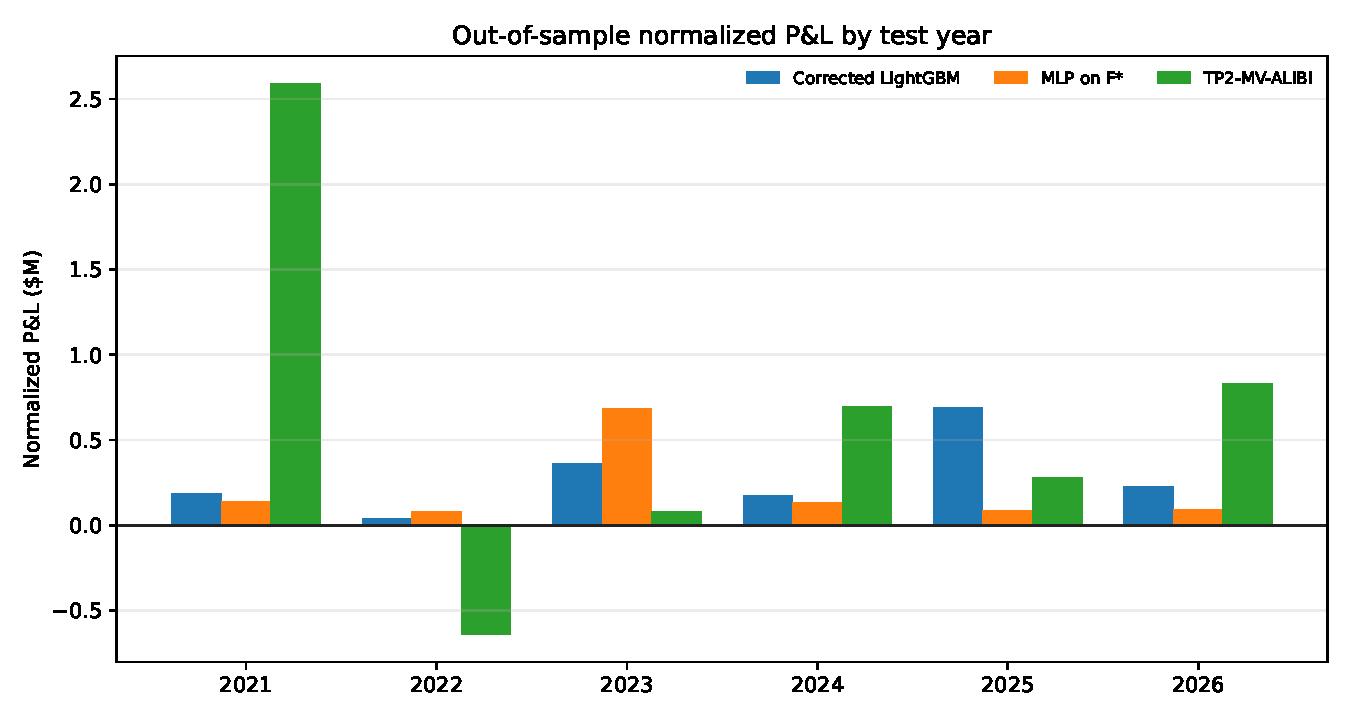
\includegraphics[width=0.94\linewidth]{figures/yearly_pnl_comparison.pdf}
\caption{Year-wise out-of-sample normalized P\&L. The transformer has larger aggregate P\&L but a clear 2022 loss, so robustness still needs work.}
\end{figure}

\begin{figure}[H]
\centering
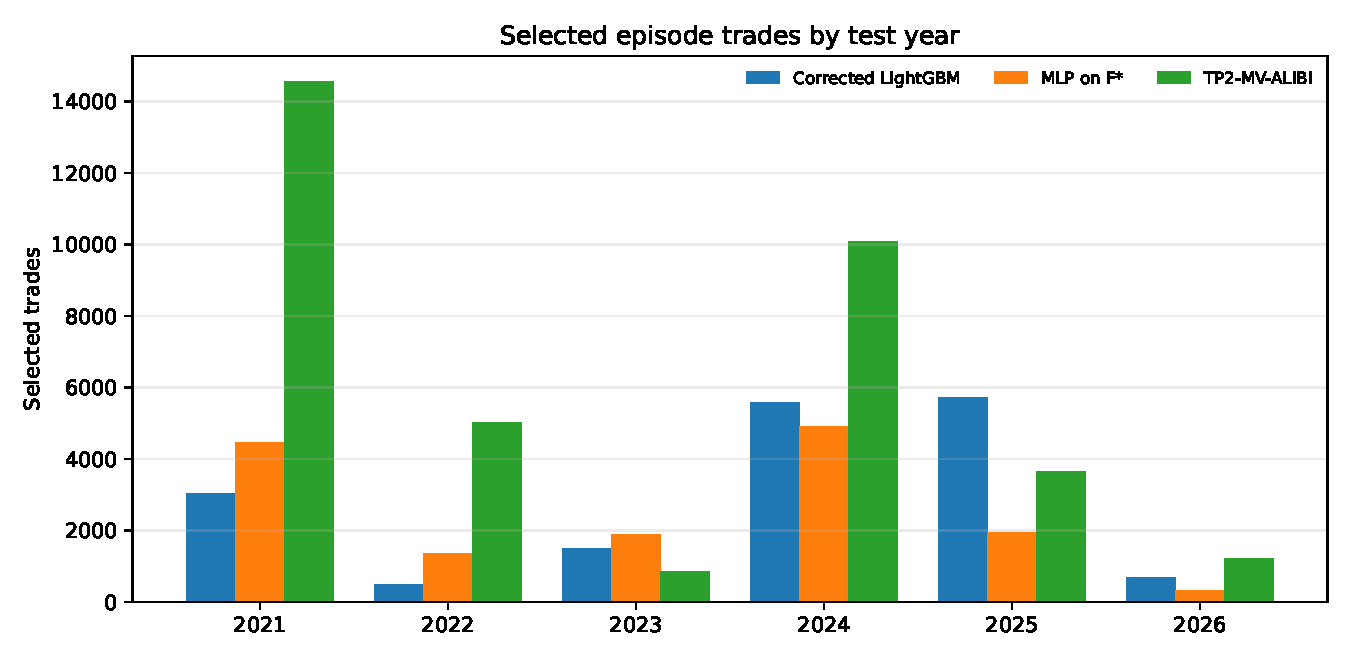
\includegraphics[width=0.94\linewidth]{figures/selected_trades_comparison.pdf}
\caption{Selected episode trades by year. The transformer currently trades more aggressively than the corrected LightGBM selector.}
\end{figure}

\begin{figure}[H]
\centering
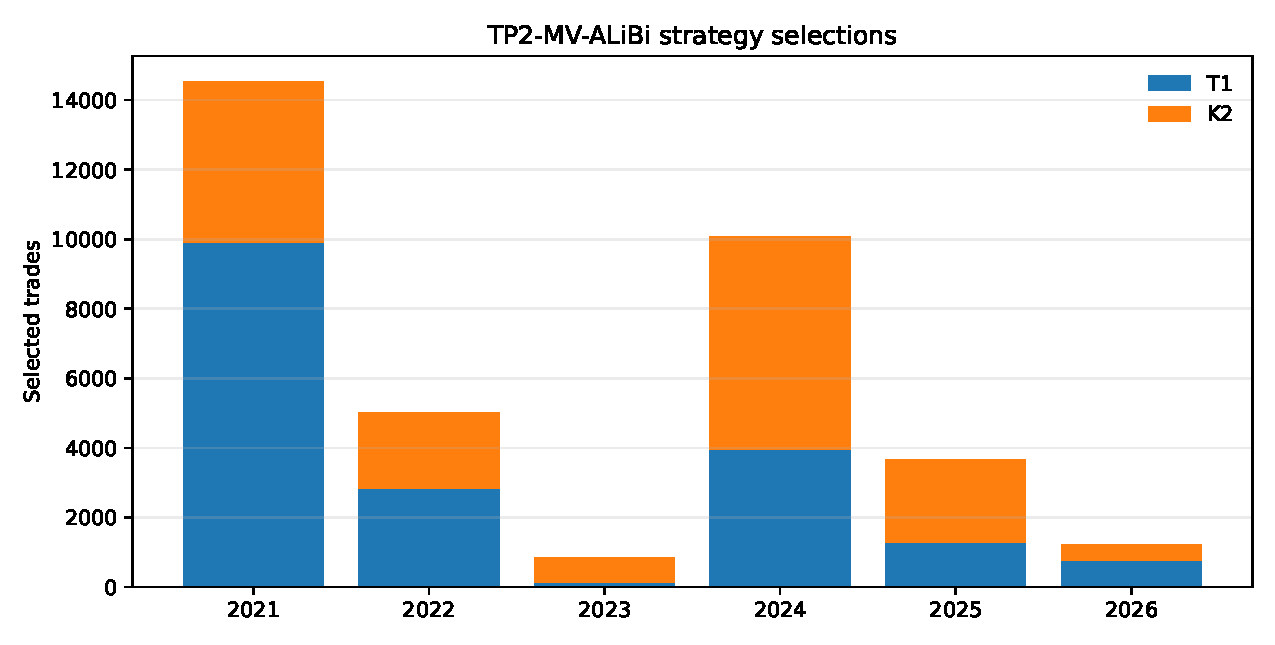
\includegraphics[width=0.86\linewidth]{figures/mv_alibi_strategy_mix.pdf}
\caption{Transformer-selected strategy mix. Only \(T1\) and \(K2\) are eligible.}
\end{figure}

\section{Transformer result}
The current TP2-MV-ALiBi run selected 35,354 trades with total normalized P\&L of \$3,839,180. It produced positive P\&L in 5 of 6 test years. The combined daily Sharpe from selected transformer trades is 1.61, and the selected-trade win rate is 34.9\%.

This should be treated as a first implemented transformer baseline, not the final conference result. The model is intentionally compact for CPU execution: it attends to the most recent 32 prior TP2 strategy tokens. The important scientific result is that the professor's architecture now runs end-to-end on our corrected labels and rolling protocol.

\section{Current caveats and next work}
\begin{itemize}
    \item The transformer improves aggregate normalized P\&L versus the current MLP ablation and the saved corrected LightGBM yearly CSV, but 2022 is negative and must be diagnosed before claiming robustness.
    \item The first transformer uses fixed-size recent-history retrieval. The next version should add ablations: no-bias transformer, time-only ALiBi, time+surface, time+surface+short-D, and full multivariate bias.
    \item Threshold selection is validation-only and therefore leakage-safe, but the low selected-trade win rate means the model is relying on large winners. We need tail-risk diagnostics and capped-return robustness.
    \item The old \texttt{ExpiryMLCorrection/meta\_selector\_clean\_summary.json} appears stale relative to its yearly CSV; this report recomputes comparison totals from the yearly result table.
\end{itemize}

\section{Files produced}
\begin{itemize}
    \item \texttt{TP2MVTransformer/data/tp2\_t1k2\_token\_dataset.parquet}
    \item \texttt{TP2MVTransformer/tables/feature\_dictionary.csv}
    \item \texttt{TP2MVTransformer/tables/mlp\_baseline\_results.csv}
    \item \texttt{TP2MVTransformer/tables/mv\_alibi\_transformer\_results.csv}
    \item \texttt{TP2MVTransformer/data/mv\_alibi\_transformer\_test\_predictions.parquet}
\end{itemize}

\end{document}
